% =============================================================================
% CHAPTER 01 -- Insurance Claims Dashboard
% =============================================================================
% Source: projects/01-insurance-claims-dashboard/
% Key files:
%   data-pipeline/01_download_cas.py      -- CAS data acquisition
%   data-pipeline/02_clean_triangles.py   -- triangle cleaning
%   data-pipeline/03_generate_claims.py   -- synthetic claim generation
%   data-pipeline/04_compute_reserves.py  -- chain-ladder + BF methods
%   sql/01_claims_summary.sql             -- portfolio snapshot
%   sql/02_loss_ratio_by_lob.sql          -- profitability analysis
%   sql/03_frequency_severity.sql         -- pure premium decomposition
%   sql/04_triangle_pivot.sql             -- triangle pivoting + factors
%   sql/05_combined_ratio.sql             -- combined ratio computation
%   backend/insurance_backend/main.py     -- FastAPI entry point
%   backend/insurance_backend/routers/    -- 5 API routers
%   src/components/insurance/            -- Next.js frontend components
% =============================================================================

\chapter{Insurance Claims Dashboard}
\label{ch:insurance}

\begin{keyinsight}
This project answers the two questions every P\&C insurance CFO needs to know:
\emph{Are we reserving enough?} and \emph{Are we pricing correctly?}
It applies two actuarial reserving methods -- Chain-Ladder and
Bornhuetter-Ferguson -- to real NAIC Schedule P regulatory data,
decomposing losses across six lines of business (LOBs) over accident years
1988--1997.  The project is the most actuarially rigorous in the portfolio
and is the natural bridge between the UNAM actuarial science curriculum and
data-analyst practice.
\end{keyinsight}

% -----------------------------------------------------------------------------
\section{Business Context}
\label{sec:ins-context}
% -----------------------------------------------------------------------------

\sourcefiles{%
  \filepath{README.md},
  \filepath{data-pipeline/04\_compute\_reserves.py}
}

A property-and-casualty (P\&C) insurer collects premiums today and pays
claims tomorrow -- sometimes years or decades later.  The regulatory and
financial reporting challenge is to estimate, at any given \emph{valuation
date}, how much has been incurred but not yet paid.  This quantity is called
the \textbf{IBNR reserve} (Incurred But Not Reported), and it flows directly
onto the insurer's balance sheet as a liability.

\paragraph{The CFO's question.}
``How much should we be holding in reserve for unpaid claims, and which lines
of business are actually profitable?''  This question requires both
\emph{actuarial reserving} (estimating future claim payments) and
\emph{profitability analysis} (comparing those estimates to earned premium).

\paragraph{Regulatory context.}
In the United States, every P\&C insurer must file \textbf{NAIC Schedule P}
as part of its annual statement.  Schedule P reports cumulative paid and
incurred losses by accident year and development lag for each line of
business -- exactly the data structure needed to build loss triangles.  The
CAS Loss Reserving Database is a publicly available dataset of historical
Schedule P filings, making it ideal for a reproducible analytical project.

\paragraph{Why this matters for an actuary.}
Reserve adequacy is an existential question for insurers.  Under-reserving
produces inflated earnings and potential insolvency; over-reserving
unnecessarily constrains capital deployment.  State insurance departments,
rating agencies (AM Best, S\&P), and auditors all scrutinize reserve
adequacy.  An actuarial science graduate entering a data-analyst role at an
insurer, reinsurer, or consulting firm will encounter loss triangles and
combined ratio analysis in the first week.

% -----------------------------------------------------------------------------
\section{CAS Loss Reserving Database}
\label{sec:ins-cas-data}
% -----------------------------------------------------------------------------

\sourcefiles{%
  \filepath{data-pipeline/01\_download\_cas.py},
  \filepath{data-pipeline/02\_clean\_triangles.py}
}

The data originates from the Casualty Actuarial Society's publicly hosted
repository of NAIC Schedule P filings.  Six CSV files are downloaded directly
from \texttt{casact.org}:

\begin{center}
\begin{tabular}{lll}
\toprule
\textbf{Filename} & \textbf{LOB} & \textbf{Actuarial tail} \\
\midrule
\texttt{ppauto\_pos.csv}   & Private Passenger Auto  & Short \\
\texttt{comauto\_pos.csv}  & Commercial Auto         & Medium \\
\texttt{wkcomp\_pos.csv}   & Workers Compensation    & Long \\
\texttt{medmal\_pos.csv}   & Medical Malpractice     & Very long \\
\texttt{othliab\_pos.csv}  & Other Liability         & Long \\
\texttt{prodliab\_pos.csv} & Product Liability       & Long \\
\bottomrule
\end{tabular}
\end{center}

\paragraph{Schema.}
Each row in the raw CSV represents one company-accident year-development year
observation.  The key columns are:

\begin{itemize}
  \item \texttt{GRCODE} / \texttt{GRNAME} -- company identifier
  \item \texttt{AccidentYear} -- the year the loss event occurred (1988--1997)
  \item \texttt{DevelopmentYear} -- the calendar year of the evaluation
  \item \texttt{DevelopmentLag} -- \texttt{DevelopmentYear - AccidentYear + 1}
    (1 = first 12 months of development, 10 = tenth year)
  \item \texttt{IncurLoss} -- cumulative incurred losses (paid + case reserves)
  \item \texttt{CumPaidLoss} -- cumulative paid losses
  \item \texttt{EarnedPremDIR} -- direct earned premium
\end{itemize}

\paragraph{Data quirk: column suffixes.}
Each CAS file uses a \emph{different} suffix on the numeric columns (e.g.,
\texttt{IncurLoss\_B}, \texttt{IncurLoss\_C}, \texttt{IncurLoss\_F2}).  The
cleaning script \filepath{02\_clean\_triangles.py} detects the suffix by
inspecting the \texttt{IncurLoss*} column name and strips it uniformly,
enabling a single code path for all six files.

\paragraph{Company selection.}
The full dataset contains roughly 30 companies per LOB.  To keep the analysis
tractable and representative, the pipeline selects the top 5 companies per LOB
by total earned premium (\texttt{COMPANIES\_PER\_LOB = 5}), yielding
approximately 3,000 triangle rows in \filepath{data/processed/triangles.parquet}.

\paragraph{Valuation date.}
Although the CAS data extends through 2006 (enabling comparison to known
ultimate outcomes), the reserving analysis truncates development at
\texttt{DevelopmentYear <= 1997}.  This simulates the perspective of an
actuary evaluating reserves \emph{as of 12/31/1997} -- the methodologically
honest way to demonstrate that the projections are out-of-sample predictions,
not fitted values.

% -----------------------------------------------------------------------------
\section{Synthetic Claims Generation}
\label{sec:ins-synthetic}
% -----------------------------------------------------------------------------

\sourcefiles{%
  \filepath{data-pipeline/03\_generate\_claims.py}
}

Schedule P is aggregate data: one row per company-accident year-development
year.  There are no individual claim records.  To build the claim-level
visualizations shown on the dashboard (severity distributions, report lag
histograms, open/closed status charts), the pipeline generates approximately
\textbf{50,000 synthetic claims} calibrated to match the CAS aggregate
patterns.

\subsection{Distributional Assumptions}

\paragraph{Severity -- LogNormal model.}
Claim severity (the loss amount per claim) is modeled as:
\begin{equation}
  S \sim \mathrm{LogNormal}(\mu, \sigma)
  \label{eq:lognormal-severity}
\end{equation}
The LogNormal distribution is standard practice for claim severity because
loss amounts are always positive, right-skewed (a few very large claims
dominate total losses), and multiplicative effects (inflation, social
inflation) are natural in log space.  Each LOB has calibrated parameters:

\begin{center}
\begin{tabular}{lcc}
\toprule
\textbf{LOB} & $\boldsymbol{\mu}$ & $\boldsymbol{\sigma}$ \\
\midrule
Private Passenger Auto  & 8.5  & 1.2 \\
Commercial Auto         & 9.0  & 1.4 \\
Workers Compensation    & 9.2  & 1.3 \\
Medical Malpractice     & 10.5 & 1.8 \\
Other Liability         & 9.5  & 1.6 \\
Product Liability       & 10.0 & 1.7 \\
\bottomrule
\end{tabular}
\end{center}

Medical Malpractice has both the highest mean ($\mu = 10.5$, median severity
$\approx e^{10.5} \approx \$36{,}000$) and highest dispersion ($\sigma = 1.8$),
reflecting its long-tail, high-severity nature.

\paragraph{Frequency -- Poisson process.}
The number of claims per LOB per accident year follows a Poisson distribution
(constant rate), an appropriate model for independent, relatively rare events.
The total target is 50,000 claims, allocated across LOBs by weight:
30\% Auto, 25\% Workers Comp, 15\% Commercial Auto, 12\% Other Liability,
10\% Med Mal, and 8\% Product Liability.

\paragraph{Report lag -- Shifted exponential.}
The delay between accident date and report date is a critical driver of IBNR.
Each claim's report lag is drawn from:
\begin{equation}
  L \sim \mathrm{Exponential}\!\left(\lambda = \frac{1}{\bar{L}}\right)
  \label{eq:report-lag}
\end{equation}
where $\bar{L}$ is the mean report lag in days.  Auto claims report quickly
($\bar{L} = 30$ days) while Medical Malpractice claims take much longer
($\bar{L} = 90$ days), producing significantly more IBNR for that LOB.

\paragraph{Settlement time -- Gamma distribution.}
The time from report to claim closure follows:
\begin{equation}
  T \sim \mathrm{Gamma}(\alpha, \beta)
  \label{eq:settlement-gamma}
\end{equation}
with shape $\alpha$ and scale $\beta$ (in days) calibrated by LOB.  For
Medical Malpractice, $\alpha = 4.0$ and $\beta = 365$ days, yielding a mean
settlement time of $4 \times 365 = 1{,}460$ days (4 years).

\paragraph{Open/closed status.}
A claim is \texttt{Closed} if its projected close date (report date plus
settlement days) falls on or before the 12/31/1997 valuation date; otherwise
it is \texttt{Open} with a case reserve equal to \texttt{incurred - paid}.

\begin{decisionbox}
\textbf{Why not use real claim data?}  Individual claim records from NAIC
Schedule P are not publicly available -- only the aggregated triangles.
Synthetic data generated from actuarially-realistic distributions allows the
dashboard to demonstrate claim-level insights (report lag analysis, severity
bands, status mix) that would otherwise be impossible.  The distributions are
calibrated to produce aggregate statistics consistent with the CAS data, so
the synthetic dataset is analytically honest even if not legally real.
\end{decisionbox}

% -----------------------------------------------------------------------------
\section{Loss Triangle Construction}
\label{sec:ins-triangle}
% -----------------------------------------------------------------------------

\sourcefiles{%
  \filepath{data-pipeline/04\_compute\_reserves.py},
  \filepath{sql/04\_triangle\_pivot.sql},
  \filepath{backend/insurance\_backend/routers/loss\_triangle.py}
}

\subsection{Formal Definition}

A \textbf{cumulative loss triangle} is a two-dimensional array
$C = \{C_{i,k}\}$ where:
\begin{itemize}
  \item $i \in \{1, 2, \ldots, n\}$ indexes accident years
    (here $i = 1988, \ldots, 1997$)
  \item $k \in \{1, 2, \ldots, K\}$ indexes development lags
    (here $k = 1, \ldots, 10$ years)
  \item $C_{i,k}$ is the \emph{cumulative} incurred (or paid) loss
    as of lag $k$ for accident year $i$
\end{itemize}

The triangle structure follows from the valuation date constraint:
cell $(i, k)$ is observed only when $i + k - 1 \leq$ valuation year.
This creates the characteristic upper-left populated / lower-right
missing pattern shown in Figure~\ref{fig:loss-triangle}.

\begin{figure}[h]
\centering
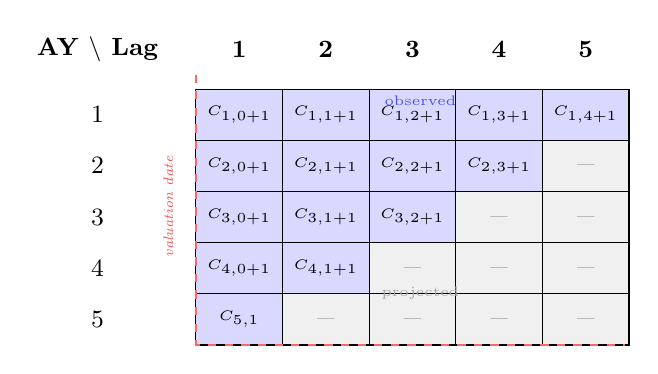
\begin{tikzpicture}[
    cell/.style={draw, minimum width=1.1cm, minimum height=0.65cm,
                 font=\tiny, inner sep=1pt},
    observed/.style={cell, fill=blue!15},
    missing/.style={cell, fill=gray!12, text=gray},
    header/.style={font=\small\bfseries},
    yearlab/.style={font=\small}
  ]

  % Column headers (development lags)
  \foreach \k/\klab in {0/1, 1/2, 2/3, 3/4, 4/5} {
    \node[header] at (1.1*\k + 1.5, 0.5) {\klab};
  }
  \node[header] at (-0.3, 0.5) {AY $\backslash$ Lag};

  % Row labels and cells
  % AY 1 -- 5 observed lags
  \node[yearlab] at (-0.3, -0.33)  {1};
  \foreach \k in {0,...,4} { \node[observed] at (1.1*\k + 1.5, -0.33) {$C_{1,\k+1}$}; }

  % AY 2 -- 4 observed lags
  \node[yearlab] at (-0.3, -0.98)  {2};
  \foreach \k in {0,...,3} { \node[observed] at (1.1*\k + 1.5, -0.98) {$C_{2,\k+1}$}; }
  \node[missing] at (1.1*4 + 1.5, -0.98) {---};

  % AY 3 -- 3 observed lags
  \node[yearlab] at (-0.3, -1.63) {3};
  \foreach \k in {0,...,2} { \node[observed] at (1.1*\k + 1.5, -1.63) {$C_{3,\k+1}$}; }
  \foreach \k in {3,...,4} { \node[missing] at (1.1*\k + 1.5, -1.63) {---}; }

  % AY 4 -- 2 observed lags
  \node[yearlab] at (-0.3, -2.28) {4};
  \foreach \k in {0,...,1} { \node[observed] at (1.1*\k + 1.5, -2.28) {$C_{4,\k+1}$}; }
  \foreach \k in {2,...,4} { \node[missing] at (1.1*\k + 1.5, -2.28) {---}; }

  % AY 5 -- 1 observed lag
  \node[yearlab] at (-0.3, -2.93) {5};
  \node[observed] at (1.5, -2.93) {$C_{5,1}$};
  \foreach \k in {1,...,4} { \node[missing] at (1.1*\k + 1.5, -2.93) {---}; }

  % Diagonal boundary annotation
  \draw[dashed, thick, red!60]
    (0.95, 0.18) -- (0.95, -3.25) -- (6.4, -3.25);

  % Labels
  \node[red!70, font=\tiny\itshape, rotate=90] at (0.6, -1.5) {valuation date};
  \node[blue!70, font=\tiny] at (3.8, -0.15) {observed};
  \node[gray!70, font=\tiny] at (3.8, -2.60) {projected};

\end{tikzpicture}
\caption{Structure of a loss development triangle. Blue cells are observed;
gray cells lie beyond the valuation date and must be projected.
The diagonal boundary represents the valuation date.}
\label{fig:loss-triangle}
\end{figure}

\subsection{From Long Format to Triangle}

The raw CAS data is in \emph{long format} (one row per accident
year $\times$ development lag). The function \texttt{build\_triangle()} in
\filepath{04\_compute\_reserves.py} pivots this into the standard matrix form
using \texttt{pandas.pivot\_table}:

\begin{lstlisting}[style=python, caption={Triangle construction in \texttt{04\_compute\_reserves.py}}]
def build_triangle(df, lob, value_col="IncurLoss"):
    lob_data = df[
        (df["line_of_business"] == lob)
        & (df["DevelopmentYear"] <= VALUATION_YEAR)   # 1997 cutoff
    ].copy()
    pivot = lob_data.pivot_table(
        index="AccidentYear",
        columns="DevelopmentLag",
        values=value_col,
        aggfunc="sum",
    )
    return pivot  # NaN in lower-right = future cells
\end{lstlisting}

The SQL equivalent is in \filepath{sql/04\_triangle\_pivot.sql}, which uses
PostgreSQL's conditional aggregation pattern to pivot lags 1--10 into
separate columns:

\begin{lstlisting}[style=sql, caption={Triangle pivot in SQL (\texttt{04\_triangle\_pivot.sql})}]
SELECT
    line_of_business, accident_year,
    MAX(incur_loss) FILTER (WHERE development_lag = 1) AS incurred_lag_01,
    MAX(incur_loss) FILTER (WHERE development_lag = 2) AS incurred_lag_02,
    -- ... lags 3-10 ...
    ROUND(incurred_lag_02 / NULLIF(incurred_lag_01, 0), 4) AS ata_01_02
FROM triangles
GROUP BY line_of_business, accident_year;
\end{lstlisting}

% -----------------------------------------------------------------------------
\section{Chain-Ladder Method}
\label{sec:ins-chain-ladder}
% -----------------------------------------------------------------------------

\sourcefiles{%
  \filepath{data-pipeline/04\_compute\_reserves.py} (lines 59--135),
  \filepath{backend/insurance\_backend/routers/loss\_triangle.py} (lines 67--93)
}

The \textbf{Chain-Ladder method} (also called the \emph{Development Method})
is the actuarial workhorse for loss reserving.  It assumes that loss
development follows a stable, repeatable pattern captured by historical
age-to-age factors.

\subsection{Age-to-Age Development Factors}

For each transition from development lag $k$ to lag $k+1$, the
\textbf{volume-weighted age-to-age factor} is:

\begin{equation}
  \hat{f}_k = \frac{\displaystyle\sum_{i:\, C_{i,k+1} \text{ observed}}
                      C_{i,k+1}}
                   {\displaystyle\sum_{i:\, C_{i,k+1} \text{ observed}}
                      C_{i,k}}
  \label{eq:ata-factor}
\end{equation}

Volume-weighting (rather than simple averaging) gives larger, more-developed
accident years greater influence -- appropriate because they represent more
statistical credibility.

\paragraph{Code implementation.}
The function \texttt{chain\_ladder()} implements Equation~\eqref{eq:ata-factor}
directly:

\begin{lstlisting}[style=python, caption={Age-to-age factor computation (\texttt{04\_compute\_reserves.py}, lines 70--88)}]
for j in range(n_lags - 1):
    col_curr = dev_lags[j]
    col_next = dev_lags[j + 1]
    numerator = 0.0
    denominator = 0.0
    for year in years:
        val_curr = triangle.loc[year, col_curr]
        val_next = triangle.loc[year, col_next]
        if pd.notna(val_curr) and pd.notna(val_next) and val_curr > 0:
            numerator += val_next
            denominator += val_curr
    factors[f"{col_curr}-{col_next}"] = numerator / denominator
\end{lstlisting}

\subsection{Cumulative Development Factors (CDFs)}

The \textbf{cumulative development factor} (CDF) from lag $k$ to ultimate
is the product of all age-to-age factors from lag $k$ onward:

\begin{equation}
  \widehat{\mathrm{CDF}}_k = \prod_{j=k}^{K-1} \hat{f}_j
  \label{eq:cdf}
\end{equation}

where $K$ is the maximum observed development lag (10 in this project).
A tail factor of 1.0 is implicitly assumed (i.e., no further development
beyond lag 10), which is conservative for short-tail lines but may
underestimate for long-tail lines like Medical Malpractice.

\begin{lstlisting}[style=python, caption={CDF computation (\texttt{04\_compute\_reserves.py}, lines 91--97)}]
factor_values = list(factors.values())
cdfs = {}
for j in range(n_lags):
    cdf = 1.0
    for k in range(j, n_lags - 1):
        cdf *= factor_values[k]
    cdfs[dev_lags[j]] = cdf
\end{lstlisting}

\subsection{Projecting Ultimate Losses}

For accident year $i$ with the latest available observation at lag $k$,
the projected ultimate loss is:

\begin{equation}
  \hat{U}_i = C_{i,k} \times \widehat{\mathrm{CDF}}_k
  \label{eq:ultimate}
\end{equation}

\subsection{IBNR Reserve Estimation}

The \textbf{IBNR reserve} for accident year $i$ is the difference between
projected ultimate and current reported losses:

\begin{equation}
  \widehat{\mathrm{IBNR}}_i = \max\!\left(0,\; \hat{U}_i - C_{i,k}\right)
  \label{eq:ibnr-cl}
\end{equation}

The $\max(0, \cdot)$ floor prevents negative IBNR from arising due to
favorable development (reserve releases).

\paragraph{Numerical example.}
For Private Passenger Auto, paid development factors
(from the \texttt{main()} output) illustrate the method:

\begin{center}
\begin{tabular}{ccc}
\toprule
\textbf{Lag transition} & \textbf{Factor} $\hat{f}_k$
  & \textbf{CDF} $\widehat{\mathrm{CDF}}_k$ \\
\midrule
1 $\to$ 2 & 1.80 & $1.80 \times \cdots$ \\
2 $\to$ 3 & 1.25 & $\cdots$ \\
$\vdots$   & $\vdots$ & $\vdots$ \\
$k \to$ ultimate & 1.00 & 1.00 \\
\bottomrule
\end{tabular}
\end{center}

The 1997 accident year has only lag-1 data available; its CDF is the
product of all nine factors, making the IBNR estimate highly leveraged
on historical patterns -- exactly why BF was developed as a complement.

\begin{keyinsight}
The portfolio's total IBNR on a paid Chain-Ladder basis is approximately
\$20.4M, with Private Passenger Auto contributing 76\% due to its volume.
Medical Malpractice carries paid CDF values of 6.1x at lag 1--2,
meaning that only 1/6.1 $\approx$ 16\% of ultimate losses have been paid
by end of year 2 -- illustrating why long-tail lines require large IBNR reserves.
\end{keyinsight}

% -----------------------------------------------------------------------------
\section{Bornhuetter-Ferguson Method}
\label{sec:ins-bf}
% -----------------------------------------------------------------------------

\sourcefiles{%
  \filepath{data-pipeline/04\_compute\_reserves.py} (lines 138--180),
  \filepath{backend/insurance\_backend/routers/loss\_triangle.py} (lines 122--145)
}

\subsection{Motivation}

The Chain-Ladder method relies entirely on observed data.  For recent
accident years (e.g., 1997, which has only one year of development),
the CL estimate is highly volatile -- a single unusual claim year
extrapolates to a large IBNR.  The \textbf{Bornhuetter-Ferguson method}
(BF) blends CL-derived development patterns with an \emph{a priori}
expected loss ratio, moderating the influence of sparse data.

\subsection{Derivation}

Partition ultimate losses into two components:
\begin{enumerate}
  \item Losses already reported (observed): $C_{i,k}$
  \item Losses yet to emerge (unreported): estimated from an a priori expectation
\end{enumerate}

The fraction of losses \emph{yet to be reported} as of lag $k$ is:
\begin{equation}
  q_k = 1 - \frac{1}{\widehat{\mathrm{CDF}}_k}
  \label{eq:pct-unreported}
\end{equation}

The \textbf{a priori expected loss} for accident year $i$ is:
\begin{equation}
  \mathrm{EL}_i = \mathrm{Premium}_i \times \mathrm{ELR}
  \label{eq:expected-loss}
\end{equation}
where ELR (\emph{expected loss ratio}) is the actuary's a priori assumption
about profitability -- typically derived from pricing actuaries, industry
benchmarks, or long-run historical averages.

The \textbf{BF IBNR} is:
\begin{align}
  \widehat{\mathrm{IBNR}}_i^{\,\mathrm{BF}}
    &= \mathrm{EL}_i \times q_k \notag \\
    &= \mathrm{Premium}_i \times \mathrm{ELR}
       \times \left(1 - \frac{1}{\widehat{\mathrm{CDF}}_k}\right)
  \label{eq:bf-ibnr}
\end{align}

The \textbf{BF ultimate} is the sum of observed losses and BF IBNR:
\begin{equation}
  \hat{U}_i^{\,\mathrm{BF}} = C_{i,k}
    + \mathrm{Premium}_i \times \mathrm{ELR}
      \times \left(1 - \frac{1}{\widehat{\mathrm{CDF}}_k}\right)
  \label{eq:bf-ultimate}
\end{equation}

\subsection{Code Implementation}

The project uses \texttt{apriori\_lr = 0.65} (65\% expected loss ratio),
a reasonable starting assumption for a mixed P\&C portfolio:

\begin{lstlisting}[style=python, caption={Bornhuetter-Ferguson (\texttt{04\_compute\_reserves.py}, lines 159--177)}]
def bornhuetter_ferguson(triangle, earned_premium, cl_cdfs,
                         apriori_lr=0.65):
    for year in sorted(triangle.index):
        latest_lag = available.index.max()
        reported   = float(available[latest_lag])
        cdf        = cl_cdfs.get(latest_lag, 1.0)
        prem       = earned_premium.get(year, 0)
        expected_loss = prem * apriori_lr

        pct_unreported = max(0, 1 - 1/cdf) if cdf > 1 else 0
        ibnr_bf        = expected_loss * pct_unreported
        ultimate_bf    = reported + ibnr_bf
\end{lstlisting}

\subsection{CL vs.\ BF Comparison}

\begin{center}
\begin{tabular}{p{4cm} p{5cm} p{5cm}}
\toprule
\textbf{Criterion} & \textbf{Chain-Ladder} & \textbf{Bornhuetter-Ferguson} \\
\midrule
Data requirement
  & Development pattern only
  & Pattern + a priori loss ratio \\
Mature years (early lags)
  & Accurate; data-rich
  & Converges to CL as $q_k \to 0$ \\
Immature years (late AYs)
  & Volatile; highly leveraged
  & Moderate; a priori anchors estimate \\
Regulatory preference
  & Standard; widely accepted
  & Often preferred for most-recent years \\
Sensitivity to one bad year
  & High (contaminates all factors)
  & Low (a priori is independent) \\
When to use
  & Long-run stable portfolios with credible history
  & New books of business; recent AYs; volatile LOBs \\
\bottomrule
\end{tabular}
\end{center}

\begin{keyinsight}
CL produces larger IBNR estimates for the most recent accident years
(1996--1997) where little development data is available; BF moderates these
projections toward the a priori expectation.  This difference is visible in
the \texttt{/api/v1/cl-vs-bf} endpoint, which returns \texttt{pct\_diff}
(the percentage by which BF IBNR differs from CL IBNR) for each accident year
and LOB.
\end{keyinsight}

% -----------------------------------------------------------------------------
\section{Profitability Analysis}
\label{sec:ins-profitability}
% -----------------------------------------------------------------------------

\sourcefiles{%
  \filepath{sql/02\_loss\_ratio\_by\_lob.sql},
  \filepath{sql/03\_frequency\_severity.sql},
  \filepath{sql/05\_combined\_ratio.sql},
  \filepath{data-pipeline/04\_compute\_reserves.py} (lines 288--294)
}

\subsection{Loss Ratio}

The \textbf{loss ratio} is the primary underwriting profitability metric:

\begin{equation}
  \mathrm{LR}_i = \frac{\text{Incurred Losses}_i}{\text{Earned Premium}_i}
  \label{eq:loss-ratio}
\end{equation}

An LR below 100\% means the line collected more premium than it paid in
losses (before expenses).  The SQL in \filepath{02\_loss\_ratio\_by\_lob.sql}
computes both a reported LR and an ultimate LR (using CL projections):

\begin{lstlisting}[style=sql, caption={Loss ratio computation (\texttt{02\_loss\_ratio\_by\_lob.sql})}]
annual_loss_ratio AS (
    SELECT
        line_of_business, accident_year,
        ROUND(100.0 * incur_loss
              / NULLIF(earned_prem_net, 0), 2) AS loss_ratio_pct,
        -- Rolling 3-year average to smooth volatility
        ROUND(AVG(loss_ratio_pct) OVER (
            PARTITION BY line_of_business
            ORDER BY accident_year
            ROWS BETWEEN 2 PRECEDING AND CURRENT ROW
        ), 2)                                  AS rolling_3yr_lr_pct
    FROM latest_eval
)
\end{lstlisting}

Profitability flags are assigned: \texttt{PROFITABLE} ($< 100\%$),
\texttt{MARGINAL} (90--100\%), \texttt{UNPROFITABLE} ($> 100\%$).

\subsection{Combined Ratio}

The \textbf{combined ratio} is the gold-standard underwriting metric,
incorporating both claim costs and operational expenses:

\begin{equation}
  \mathrm{CR} = \mathrm{LR} + \mathrm{ER}
  = \frac{\text{Incurred Losses} + \text{Expenses}}{\text{Earned Premium}}
  \label{eq:combined-ratio}
\end{equation}

where ER is the expense ratio.  A CR below 100\% means underwriting profit;
above 100\% means the insurer relies on investment income to be profitable.

\begin{center}
\begin{tabular}{ll}
\toprule
\textbf{Combined Ratio} & \textbf{Interpretation} \\
\midrule
$< 95\%$   & Strong underwriting profit \\
$95-100\%$ & Marginal profit \\
$100-110\%$ & Marginal loss; investment income may compensate \\
$> 110\%$  & Significant loss \\
\bottomrule
\end{tabular}
\end{center}

The project assumes a flat 30\% expense ratio (U.S. industry average for P\&C):
\begin{equation}
  \mathrm{CR} = \mathrm{LR} + 0.30
  \label{eq:combined-ratio-assumed}
\end{equation}

This assumption is made explicit in the SQL via a \texttt{params} CTE
to facilitate sensitivity analysis.

\subsection{Frequency-Severity Decomposition}

The fundamental identity of insurance pricing:

\begin{equation}
  \text{Pure Premium} = \text{Frequency} \times \text{Severity}
  \label{eq:pure-premium}
\end{equation}

where:
\begin{align}
  \text{Frequency} &= \frac{\text{Claim Count}}{\text{Exposure}}
  \label{eq:frequency} \\
  \text{Severity}  &= \frac{\text{Total Losses}}{\text{Claim Count}}
  \label{eq:severity}
\end{align}

This decomposition is critical for claims management decisions:
rising frequency signals underwriting/risk selection problems;
rising severity signals claims management or trend issues.

The SQL in \filepath{03\_frequency\_severity.sql} computes year-over-year
growth rates for both components and flags the \emph{primary loss driver}:

\begin{lstlisting}[style=sql, caption={Loss driver identification (\texttt{03\_frequency\_severity.sql})}]
CASE
    WHEN ABS(frequency_yoy_pct) > ABS(severity_yoy_pct)
        THEN 'FREQUENCY DRIVEN'
    WHEN ABS(severity_yoy_pct) > ABS(frequency_yoy_pct)
        THEN 'SEVERITY DRIVEN'
    ELSE 'BALANCED'
END AS primary_loss_driver
\end{lstlisting}

Since the project uses synthetic claims, exposure is proxied by earned premium,
yielding a \emph{pure premium rate} (loss per dollar of premium) rather than
traditional frequency per policy.

\begin{keyinsight}
From the README findings:
\textbf{Private Passenger Auto} and \textbf{Product Liability} are the only
profitable lines (combined ratio $< 100\%$).  \textbf{Medical Malpractice}
shows the highest loss ratio ($\approx 280\%$) with the longest development
tails -- claims take 3--5$\times$ longer to report than Auto, creating the
largest IBNR uncertainty of all six LOBs.
\end{keyinsight}

% -----------------------------------------------------------------------------
\section{System Architecture}
\label{sec:ins-architecture}
% -----------------------------------------------------------------------------

\sourcefiles{%
  \filepath{backend/insurance\_backend/main.py},
  \filepath{backend/insurance\_backend/data\_loader.py},
  \filepath{src/components/insurance/InsuranceDashboard.tsx}
}

\subsection{4-Stage ETL Pipeline}

\begin{center}
\begin{tikzpicture}[
    node distance=0.4cm,
    box/.style={draw, rounded corners=3pt, minimum width=3.2cm,
                minimum height=0.9cm, align=center, font=\small,
                fill=blue!8, draw=blue!40},
    arrow/.style={-{Stealth[length=5pt]}, thick, blue!50}
  ]

  \node[box] (s1) {\textbf{Stage 1}\\Download CAS CSVs};
  \node[box, right=of s1] (s2) {\textbf{Stage 2}\\Clean Triangles};
  \node[box, right=of s2] (s3) {\textbf{Stage 3}\\Generate Claims};
  \node[box, right=of s3] (s4) {\textbf{Stage 4}\\Compute Reserves};

  \draw[arrow] (s1) -- (s2);
  \draw[arrow] (s2) -- (s3);
  \draw[arrow] (s3) -- (s4);

  % Output labels
  \node[font=\tiny, gray, below=0.1cm of s1] {\texttt{data/raw/*.csv}};
  \node[font=\tiny, gray, below=0.1cm of s2] {\texttt{triangles.parquet}};
  \node[font=\tiny, gray, below=0.1cm of s3] {\texttt{claims\_synthetic.parquet}};
  \node[font=\tiny, gray, below=0.1cm of s4] {\texttt{ibnr\_results.parquet}};

\end{tikzpicture}
\end{center}

\begin{description}
  \item[Stage 1 -- \filepath{01\_download\_cas.py}]
    Downloads six CAS CSVs from \texttt{casact.org}.  Idempotent: skips files
    that already exist.

  \item[Stage 2 -- \filepath{02\_clean\_triangles.py}]
    Detects and strips per-file column suffixes, tags each row with a
    human-readable LOB name, selects top 5 companies per LOB by premium volume,
    and computes derived columns (\texttt{loss\_ratio},
    \texttt{paid\_to\_incurred}).
    Output: \filepath{data/processed/triangles.parquet}.

  \item[Stage 3 -- \filepath{03\_generate\_claims.py}]
    Generates 50,000 synthetic claims using LOB-calibrated lognormal severity,
    exponential report lag, and gamma settlement distributions.
    Output: \filepath{data/processed/claims\_synthetic.parquet}.

  \item[Stage 4 -- \filepath{04\_compute\_reserves.py}]
    Builds valuation-date triangles for both incurred and paid bases, runs
    chain-ladder on each, runs BF on paid losses with \texttt{apriori\_lr = 0.65},
    and aggregates LOB-level summaries.
    Outputs: \filepath{data/processed/ibnr\_results.parquet} and
    \filepath{data/processed/lob\_summary.parquet}.
\end{description}

\subsection{FastAPI Backend}

The backend loads all four parquet files at startup via
\filepath{backend/insurance\_backend/data\_loader.py} and exposes five API
routers under the \texttt{/api/v1} prefix:

\begin{center}
\begin{tabular}{ll}
\toprule
\textbf{Router module} & \textbf{Endpoint} \\
\midrule
\texttt{loss\_triangle.py}        & \texttt{GET /api/v1/loss-triangle} \\
                                  & \texttt{GET /api/v1/cl-vs-bf} \\
\texttt{frequency\_severity.py}   & \texttt{GET /api/v1/frequency-severity} \\
\texttt{loss\_ratios.py}          & \texttt{GET /api/v1/loss-ratios} \\
\texttt{combined\_ratio.py}       & \texttt{GET /api/v1/combined-ratio} \\
\texttt{claim\_distribution.py}   & \texttt{GET /api/v1/claim-distribution} \\
\bottomrule
\end{tabular}
\end{center}

All endpoints accept optional query parameters \texttt{lob}, \texttt{company},
\texttt{year\_start}, and \texttt{year\_end} for dashboard filtering.
The \texttt{/api/v1/loss-triangle} endpoint additionally accepts
\texttt{type} (\texttt{incurred}/\texttt{paid}) and \texttt{method}
(\texttt{cl}/\texttt{bf}), computing CL factors on-the-fly from the filtered
triangle and overriding the IBNR estimates from the pre-computed parquet when
BF is requested.

\subsection{Next.js Frontend}

The dashboard runs at \texttt{localhost:3051} and proxies all API calls through
Next.js rewrites to avoid CORS issues.  Browser traffic never reaches the
FastAPI port directly.

Key React components in
\filepath{src/components/insurance/}:

\begin{itemize}
  \item \texttt{LossTriangleHeatmap.tsx} -- interactive heatmap; toggle
    incurred/paid and CL/BF
  \item \texttt{IBNRWaterfall.tsx} -- waterfall: Paid + Case Reserve + IBNR = Ultimate
  \item \texttt{FrequencySeverityChart.tsx} -- dual-axis: claim count (bars)
    and avg severity (line)
  \item \texttt{LossRatioByLOB.tsx} -- reported vs.\ ultimate LR bar chart
  \item \texttt{CombinedRatioTrend.tsx} -- stacked area: loss ratio + expense ratio
  \item \texttt{CLvsBFTable.tsx} -- tabular comparison of CL and BF IBNR by year
  \item \texttt{InsuranceFilterBar.tsx} -- LOB / company / year-range selectors
\end{itemize}

\begin{decisionbox}
\textbf{Why Next.js instead of Power BI?}
Power BI was the original plan, but it requires a Windows machine with PBI
Desktop and a licensed workspace for embedding.  Next.js + Recharts gives
full control over dark/light theming (the dashboard supports both modes with
LOB-specific CSS variables like \texttt{--lob-auto}, \texttt{--lob-workers}),
a static export that merges into the shared portfolio hub, and the ability to
call FastAPI endpoints through an edge proxy rather than exposing them.  The actuarial calculations remain in Python,
which is far more transparent than DAX measures.
\end{decisionbox}

% -----------------------------------------------------------------------------
\section{SQL Queries}
\label{sec:ins-sql}
% -----------------------------------------------------------------------------

\sourcefiles{%
  \filepath{sql/01\_claims\_summary.sql},
  \filepath{sql/02\_loss\_ratio\_by\_lob.sql},
  \filepath{sql/03\_frequency\_severity.sql},
  \filepath{sql/04\_triangle\_pivot.sql},
  \filepath{sql/05\_combined\_ratio.sql}
}

Five analytical SQL queries cover the full story from raw claims to
underwriting decision support.  All are written in PostgreSQL dialect with
CTEs for readability.

\paragraph{Query 01 -- Claims portfolio snapshot.}
\emph{Business question: What does our claims landscape look like by LOB and status?}

Produces count, open/closed split, average severity (paid and incurred),
total case reserves, and severity-band distribution per LOB.
Uses three CTEs: \texttt{claims\_by\_lob\_status} $\to$
\texttt{lob\_pivot} (conditional sums for open/closed) $\to$
\texttt{portfolio\_totals} (UNION ALL grand total row).
Key pattern: \texttt{NULLIF(denominator, 0)} guards every division.

\paragraph{Query 02 -- Loss ratio by LOB.}
\emph{Business question: Which lines of business are profitable?}

Joins triangles (most mature lag per accident year via \texttt{DISTINCT ON})
to \texttt{ibnr\_results} for ultimate loss ratios.  Adds a rolling 3-year
window average:

\begin{lstlisting}[style=sql, caption={Rolling window loss ratio (\texttt{02\_loss\_ratio\_by\_lob.sql})}]
AVG(loss_ratio_pct) OVER (
    PARTITION BY line_of_business
    ORDER BY accident_year
    ROWS BETWEEN 2 PRECEDING AND CURRENT ROW
) AS rolling_3yr_lr_pct
\end{lstlisting}

Assigns \texttt{CHRONIC ISSUE} when the rolling 3-year average exceeds 100\%,
directing management attention to persistently unprofitable lines.

\paragraph{Query 03 -- Frequency-severity decomposition.}
\emph{Business question: Are losses driven by more claims or larger claims?}

Joins \texttt{claims\_synthetic} to \texttt{triangles} for an exposure proxy,
computes frequency per \$1M of earned premium and incurred severity, then
uses \texttt{LAG()} window functions to produce year-over-year growth rates.
The \texttt{primary\_loss\_driver} flag guides management action:
frequency-driven losses suggest underwriting intervention; severity-driven
losses suggest claims management improvements.

\paragraph{Query 04 -- Triangle pivot.}
\emph{Business question: What does the loss development pattern look like?}

Pivots the long-format triangles table into the standard actuarial wide
layout using \texttt{FILTER (WHERE development\_lag = k)} conditional
aggregation.  Also computes individual age-to-age factors per accident year
and volume-weighted average factors in a separate CTE -- the equivalent of
what the Python chain-ladder code does, but expressible in pure SQL.

\paragraph{Query 05 -- Combined ratio analysis.}
\emph{Business question: Is the portfolio profitable after expenses?}

Uses a \texttt{params} CTE (\texttt{assumed\_expense\_ratio = 0.30}) to
make the flat expense assumption explicit and easy to change.  Computes
reported CR, ultimate CR (including IBNR from chain-ladder), a 3-year rolling
CR, and year-over-year CR change.  Profitability bands (\texttt{STRONG PROFIT}
through \texttt{SIGNIFICANT LOSS}) and trend flags (\texttt{IMPROVING},
\texttt{DETERIORATING}, \texttt{STABLE}) provide dashboard-ready text labels.

% -----------------------------------------------------------------------------
\section{Challenge and Interview Questions}
\label{sec:ins-questions}
% -----------------------------------------------------------------------------

\begin{challengebox}
\textbf{Triangle completeness and the valuation date.}
The code sets \texttt{VALUATION\_YEAR = 1997}.  If you moved the valuation
date to 1993, which cells in the triangle would be removed?  How would the
chain-ladder factors change, and in which direction would IBNR estimates
move for the 1993 accident year?  Explain using Equation~\eqref{eq:ata-factor}.
\end{challengebox}

\begin{challengebox}
\textbf{Tail factor sensitivity.}
The project assumes a tail factor of 1.000 beyond lag 10 for all LOBs.
For Medical Malpractice (a very long-tail line), this is arguably wrong.
If you applied a tail factor of 1.15 (15\% additional development beyond lag 10),
how would the IBNR change for the oldest accident year (1988)?  Show the
algebraic adjustment to Equations~\eqref{eq:cdf} and \eqref{eq:ultimate}.
\end{challengebox}

\begin{challengebox}
\textbf{BF convergence.}
Prove algebraically that as $k \to K$ (i.e., as an accident year approaches
full development), the BF ultimate in Equation~\eqref{eq:bf-ultimate}
converges to the observed value $C_{i,K}$.  What does this imply about when
BF and CL agree?
\end{challengebox}

\begin{challengebox}
\textbf{Volume weighting vs.\ simple average.}
The code computes volume-weighted factors (Equation~\eqref{eq:ata-factor}).
Construct a numerical example with three accident years where the simple-average
factor and the volume-weighted factor differ by more than 10\%.  Which is
more appropriate and why?  When might an actuary deliberately choose a simple
average or an ``all-but-one-year'' factor selection?
\end{challengebox}

\begin{interviewbox}
\textbf{Explain IBNR to a non-actuarial CFO.}
The CFO asks: ``Our loss triangle shows \$15M of paid losses.  Your report
says our ultimate is \$20.4M.  Where did the extra \$5.4M come from, and
do we actually owe it?''  Give a 2-minute plain-language answer.
\end{interviewbox}

\begin{interviewbox}
\textbf{When would you choose BF over Chain-Ladder?}
The pricing team just launched a new commercial auto product six months ago.
You have half a year of loss data.  Which method would you use to estimate
IBNR and why?  What a priori loss ratio would you select, and where does
it come from?
\end{interviewbox}

\begin{interviewbox}
\textbf{Combined ratio interpretation.}
Medical Malpractice shows a combined ratio of approximately 310\% in this
project.  Does that mean the insurer is bankrupt?  What information would
you need to determine whether the company is financially viable despite
this underwriting loss?
\end{interviewbox}

\begin{interviewbox}
\textbf{Frequency-severity trade-offs in pricing.}
Your analysis flags a line as ``SEVERITY DRIVEN'' because average incurred
severity increased 12\% year-over-year while frequency was flat.  What are
three possible root causes of rising severity?  For each, describe the
management response that would be appropriate.
\end{interviewbox}
